%File: formatting-instructions-latex-2025.tex
%release 2025.0
\documentclass[letterpaper]{article} % DO NOT CHANGE THIS
\usepackage{aaai25}  % DO NOT CHANGE THIS
\usepackage{times}  % DO NOT CHANGE THIS
\usepackage{helvet}  % DO NOT CHANGE THIS
\usepackage{courier}  % DO NOT CHANGE THIS
\usepackage[hyphens]{url}  % DO NOT CHANGE THIS
\usepackage{graphicx} % DO NOT CHANGE THIS
\urlstyle{rm} % DO NOT CHANGE THIS
\def\UrlFont{\rm}  % DO NOT CHANGE THIS
\usepackage{natbib}  % DO NOT CHANGE THIS AND DO NOT ADD ANY OPTIONS TO IT
\usepackage{caption} % DO NOT CHANGE THIS AND DO NOT ADD ANY OPTIONS TO IT
\frenchspacing  % DO NOT CHANGE THIS
\setlength{\pdfpagewidth}{8.5in}  % DO NOT CHANGE THIS
\setlength{\pdfpageheight}{11in}  % DO NOT CHANGE THIS
%
% These are recommended to typeset algorithms but not required. See the subsubsection on algorithms. Remove them if you don't have algorithms in your paper.
\usepackage{algorithm}
\usepackage{algorithmic}

%
% These are are recommended to typeset listings but not required. See the subsubsection on listing. Remove this block if you don't have listings in your paper.
\usepackage{newfloat}
\usepackage{listings}
\DeclareCaptionStyle{ruled}{labelfont=normalfont,labelsep=colon,strut=off} % DO NOT CHANGE THIS
\lstset{%
	basicstyle={\footnotesize\ttfamily},% footnotesize acceptable for monospace
	numbers=left,numberstyle=\footnotesize,xleftmargin=2em,% show line numbers, remove this entire line if you don't want the numbers.
	aboveskip=0pt,belowskip=0pt,%
	showstringspaces=false,tabsize=2,breaklines=true}
\floatstyle{ruled}
\newfloat{listing}{tb}{lst}{}
\floatname{listing}{Listing}
%
% Keep the \pdfinfo as shown here. There's no need
% for you to add the /Title and /Author tags.
\pdfinfo{
/TemplateVersion (2025.1)
}

% DISALLOWED PACKAGES
% \usepackage{authblk} -- This package is specifically forbidden
% \usepackage{balance} -- This package is specifically forbidden
% \usepackage{color (if used in text)
% \usepackage{CJK} -- This package is specifically forbidden
% \usepackage{float} -- This package is specifically forbidden
% \usepackage{flushend} -- This package is specifically forbidden
% \usepackage{fontenc} -- This package is specifically forbidden
% \usepackage{fullpage} -- This package is specifically forbidden
% \usepackage{geometry} -- This package is specifically forbidden
% \usepackage{grffile} -- This package is specifically forbidden
% \usepackage{hyperref} -- This package is specifically forbidden
% \usepackage{navigator} -- This package is specifically forbidden
% (or any other package that embeds links such as navigator or hyperref)
% \indentfirst} -- This package is specifically forbidden
% \layout} -- This package is specifically forbidden
% \multicol} -- This package is specifically forbidden
% \nameref} -- This package is specifically forbidden
% \usepackage{savetrees} -- This package is specifically forbidden
% \usepackage{setspace} -- This package is specifically forbidden
% \usepackage{stfloats} -- This package is specifically forbidden
% \usepackage{tabu} -- This package is specifically forbidden
% \usepackage{titlesec} -- This package is specifically forbidden
% \usepackage{tocbibind} -- This package is specifically forbidden
% \usepackage{ulem} -- This package is specifically forbidden
% \usepackage{wrapfig} -- This package is specifically forbidden
% DISALLOWED COMMANDS
% \nocopyright -- Your paper will not be published if you use this command
% \addtolength -- This command may not be used
% \balance -- This command may not be used
% \baselinestretch -- Your paper will not be published if you use this command
% \clearpage -- No page breaks of any kind may be used for the final version of your paper
% \columnsep -- This command may not be used
% \newpage -- No page breaks of any kind may be used for the final version of your paper
% \pagebreak -- No page breaks of any kind may be used for the final version of your paperr
% \pagestyle -- This command may not be used
% \tiny -- This is not an acceptable font size.
% \vspace{- -- No negative value may be used in proximity of a caption, figure, table, section, subsection, subsubsection, or reference
% \vskip{- -- No negative value may be used to alter spacing above or below a caption, figure, table, section, subsection, subsubsection, or reference

\setcounter{secnumdepth}{0} %May be changed to 1 or 2 if section numbers are desired.

% The file aaai25.sty is the style file for AAAI Press
% proceedings, working notes, and technical reports.
%

% Title

% Your title must be in mixed case, not sentence case.
% That means all verbs (including short verbs like be, is, using,and go),
% nouns, adverbs, adjectives should be capitalized, including both words in hyphenated terms, while
% articles, conjunctions, and prepositions are lower case unless they
% directly follow a colon or long dash
\title{Using Knowledge-Based AI to Solve ARC-Prize Problems}
\author{
    Matthew Ellis
}
\affiliations{
    Georgia Institute of Technology
}

\begin{document}

\maketitle

% \begin{abstract}
% Lorem Ipsum Abstract
% \end{abstract}

% Uncomment the following to link to your code, datasets, an extended version or similar.
%
% \begin{links}
%     \link{Code}{https://aaai.org/example/code}
%     \link{Datasets}{https://aaai.org/example/datasets}
%     \link{Extended version}{https://aaai.org/example/extended-version}
% \end{links}

\section{Introduction}
This Autumn, Mike Knoop and Francios Chollet put up over a million dollars to entice the Artificial Intelligence community to find a new and creative solution to the problem of instilling AI models with basic reasoning and common sense. More specifically, they are looking to find ways of developing models that ``acquire new skills and solve open-ended problems'' \cite{arcprize}.

These ARC problems are represented by grids of colored squares. This way, the problems are not dependent on any specific language or culture. For any given problem, there is a set of training pairs and a test input. These training pairs include both the input and output grids, while the test only comes with an input and no output. The user/model must generate an output grid to pair with the test input.

There is no formal problem definition for any of these problems - an agent is simply supposed to examine the test pairs and deduce an output for the test input. For a human agent, this means using their intuition to recognize patterns or see a big picture that makes the answer readily apparent. However, computers struggle with these tasks as it is difficult to program a computer to handle an amorphous and vaguely defined task like this one.

The first hurdle an agent has to clear is deciding what size the output should be. For many problems, this means simply copying the size of the input grid. But for others, the size of the output could depend on latent information in the input grid itself.

The picture below on the left is a scenario where the output shape is the same as the input shape, but that is not the case for the picture on the right.

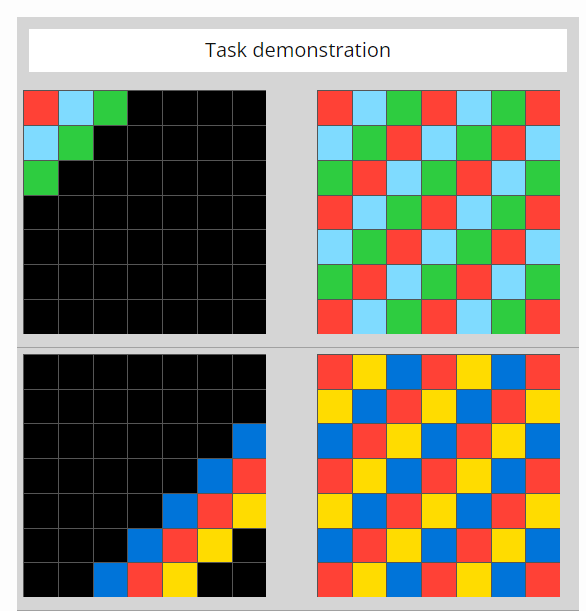
\includegraphics[scale=0.25]{ex1.png}
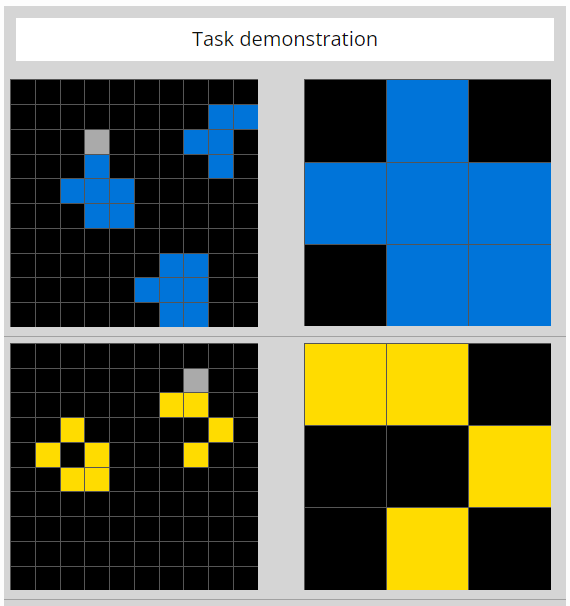
\includegraphics[scale=0.25]{ex2.png}

Based on my experience solving a few of these puzzles, my basic workflow is
\begin{enumerate}
    \item Find a pattern between the size of the test inputs and their outputs (eg outputs are the same size as their inputs, shrunk by factor of 3, etc). Use this pattern to determine the test output size.
    \item Find a common pattern that maps the training inputs to their outputs.
    \item Apply this pattern to the test input to determine its output.
\end{enumerate}

\bigskip

In an effort to narrow the scope of the ARC problems a little bit, I classified some of the problems I saw into categories:


\begin{itemize}
    \item Binary Operation\\
    This is when the input is separated into 2 halves, and the output is the result of some binary operation (AND, XOR, \ldots) on these 2 halves. \\
    \item Stationary Input Modification\\
    This is when the output is nearly identical to the input except for a few squares being changed. All the 'structures' from the input remain in tact and in the same place.\\
    \item Dynamic Input Modification\\
    In these problems, the 'structures' remain in tact but move to other locations on the grid.\\
    \item Missing Window\\
    These problems include a square of uniform color sitting on top of a image, the goal being to determine what lies underneath the square. These can be solved using symmetry from other parts of the image.\\
    \item Downsampling\\
    The output grid is a smaller version of the input image, almost like a lower-level depiction of the same fractal.\\
    \item Upsampling \\
    The output grid is a larger version of the input image, almost like a higher-level depiction of the same fractal.\\
\end{itemize}

Knowing which class a problem falls into would make solving it much simpler; implementing functions to solve each of these problem classes individually would be simpler than implementing an algorithm to solve any ARC problem.

However, this would introduce a new problem of classifying a problem as one of the 6 above, which would be far from trivial in and of itself.

\bigskip

The more I learn about the ARC problems, the more I understand why Mike Knoop and Francios Chollet put such a large bounty on its solution. These are somewhat simple problems (to humans, at least) that have no good solution at the time of writing. It seems like an elegant solution to this problem \textit{has} to exist, but finding that solution won't be easy.

\section{Related Work}
Vanilla Machine Learning approaches and LLMs have both fallen well short of the human benchmark for ARC, so researchers have come up with creative ways of representing and solving these problems.

\bigskip

Xu, Khalil, and Stanner attempted to mimic the way humans think about ARC problems using Abstract Reasoning with Graphical Abstractions, or ARGA for short \cite{Xu_Khalil_Sanner_2023}. Their algorithm first transforms the grid of pixels into a graph of objects. These objects are clusters of pixels that humans would recognize as belonging together. Then, their algorithm can apply a transformation to these objects to modify the graph. These transformations are things like rotating an object, changing its color, removing it, etc. The algorithm searches through the state space of different combinations of these transformations until it reaches the output state. Then it simply applies these transformations to the test input grid.

To make this algorithm run in a reasonable amount of time, the search is optimized with a heuristic that selects the best state to expand on and constraints that limit the size of the search space. This approach was almost able to match the performance of the 2020 ARC Prize winner while using significantly less compute resources \cite{Xu_Khalil_Sanner_2023}.

\bigskip

Xu and Khalil also attempted to use LLMs to solve the ARC tasks. The first issue they ran into was representing the task grids as text, as LLMs like ChatGPT are primed to accept text input. This yielded poor results, so the researchers opted to use their ARGA generating algorithm from the paper mentioned above to feed ChatGPT an abstract graph instead of a concrete grid of text. This led to better performance, but their model didn't even reach 50\% accuracy on the easiest ARC problems \cite{xu2024llmsabstractionreasoningcorpus}.

\bigskip

Lee et al decided to go in a different direction - they tried using Reinforcement Learning to improve their model's analogical reasoning \cite{lee2024enhancinganalogicalreasoningabstraction}. They found that model-based RL yielded solid results, but with one major caveat. They restricted their action space to only 4 transformations plus a 'submit' action in order to reduce compute complexity. Despite their promising results, it may be the case that RL isn't feasible to use on a problem as vast as the ARC Corpus.

\bigskip

Lei et al opted for yet another strategy: planning. They used the standard language for solving planning problems: Planning Domain Definition Language, or PDDL. Lei also used many strategies from Xu's 2023 paper, including abstract graph representation and argument constraints. Using this planning strategy, Lei was able to achieve an accuracy of over 50\% on the testing set, besting the previous winner's kaggle submission \cite{Lei_Lipovetzky_Ehinger_2024}.

\bigskip

In researching methods that others have used to solve the ARC problems, I also investigated some strategies around Raven's Progressive Matrices. The methods of solving these had some similar themes as the methods for solving ARC problems. Like strategies for solving ARC tasks, those for solving Raven's Progressive Matrices are composed of two main parts:
\begin{enumerate}
    \item Generate some higher-level representation of the information displayed in the problem.
    \item Infer a set of transformations and use them to deduce what the output should be.
\end{enumerate}
The paper I read about Raven's used a geometric approach to transformations, specifically affine transformations \cite{KUNDA201347}.

\bigskip

Throughout every paper I read, the key topics that kept popping back up were the 2 halves of the problem I mentioned immediately above. Multiple papers opted to solve the first half using the ARGA engine from Xu, Khalil, and Stanner 2023. This re-use of the ARGA engine leads me to believe that there is more room for improvement in step 2: transformation inference.

Thinking about the process of inferring transformations, I realized that many of the AI models in these papers perform poorly on the withheld testing set because the transformations in these tasks aren't appearing in the training set. A more robust AI model would be able to learn transformations as it goes instead of having the programmer hard code them into the source code. However, this is more easily said than done, and it may even be intractable with modern compute resources.

\section{Methodology}
My first attempt at solving the ARC Prize Problem was based on Breadth-First Search since this method is straightforward to implement and easy to understand. First, I had to find a Domain Specific Language for my algorithm to search over. I decided to reuse the actions from Homework 2 to build the DSL \cite{maclellan_arc_homework}. This DSL included only global actions---I did not implement any way to extract objects from the grids and search over object-specific actions. The actions that were encoded in the DSL are
\begin{itemize}
    \item tophalf
    \item rot90
    \item hmirror
    \item vmirror
    \item lshift
    \item compress
    \item mapcolor(a,b)
    \item trim
\end{itemize}
The pseudocode for my algorithm is described below:
\begin{algorithmic}
    \STATE $Q \gets initial \: state$
    \WHILE{$Q$ is not empty}
        \STATE $curr \: state \gets Q$.pop()
        \FORALL{$action$ $\in$ DSL}
            \STATE $new \: state \gets curr \: state$.perform$(action)$
            \IF{$new \: state = goal \: state$}
                \STATE Halt
            \ELSE
                \STATE $Q$.push$(new \; state)$
            \ENDIF
        \ENDFOR
    \ENDWHILE
\end{algorithmic}

\bigskip

I have also included the following visual representation of this algorithm
\begin{center}
    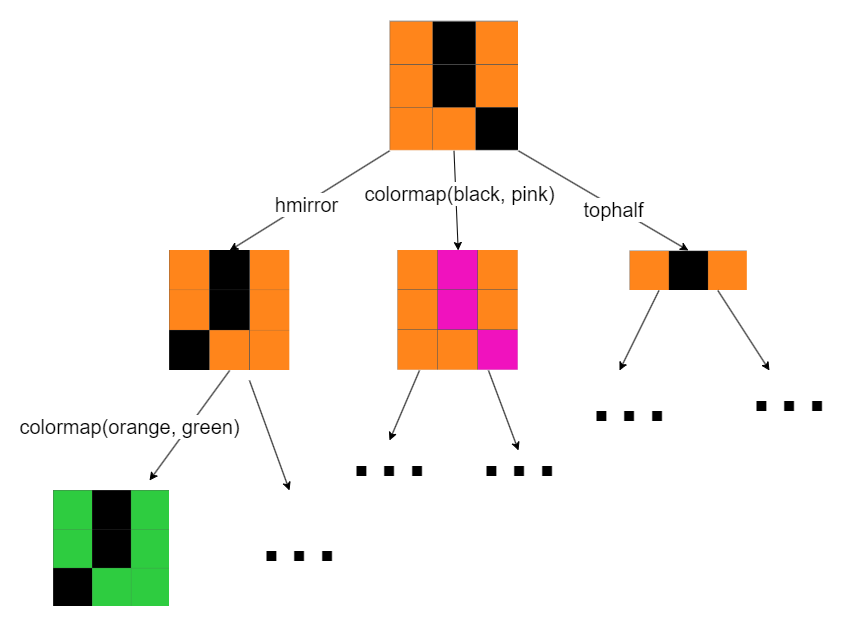
\includegraphics[width=\hsize]{BFS_tree.drawio.png}
\end{center}

\bigskip

This algorithm finds the chain of actions, which I will call the transformation, that transforms the initial state into the goal state. I also included a few optimizations in my implementation of this algorithm so that it would run in a reasonable amount of time.
\begin{itemize}
    \item Limit the depth of the search to 2 layers past the root
    \item Refuse to expand/revisit puzzle states that have already been added to the queue
    \item Only consider mapcolor($a$, $b$) if $a$ and $b$ actually show up in the input grid or output grid
\end{itemize}

\bigskip

Once the algorithm has inferred a transformation based on the training pair(s), it applies that transformation to the testing input(s) and submits the output. If the algorithm cannot infer a transformation that transforms the testing inputs into their respective outputs, then it infers the null transformation and simply returns the testing input(s) with no modifications.

\bigskip

If the algorithm infers multiple conflicting transformations from the training pairs, then it prefers to select the longer transformation so that it is biased away from null transformations.

\section{Experiments}
After running the BFS algorithm a few times on the evaluation set, it has returned scores anywhere from 1.5 to 4 out of 400, and it takes about 40 seconds to process all 400 problems.

\bigskip

I found it interesting that my algorithm wasn't deterministic---the score changed between executions even though I didn't change any of the code. My best guess for what causes this is that my algorithm is arbitrarily breaking ties between conflicting transformations of the same length.

\bigskip

I've included some ARC tasks that my algorithm was successfully able to solve below:

\begin{center}
    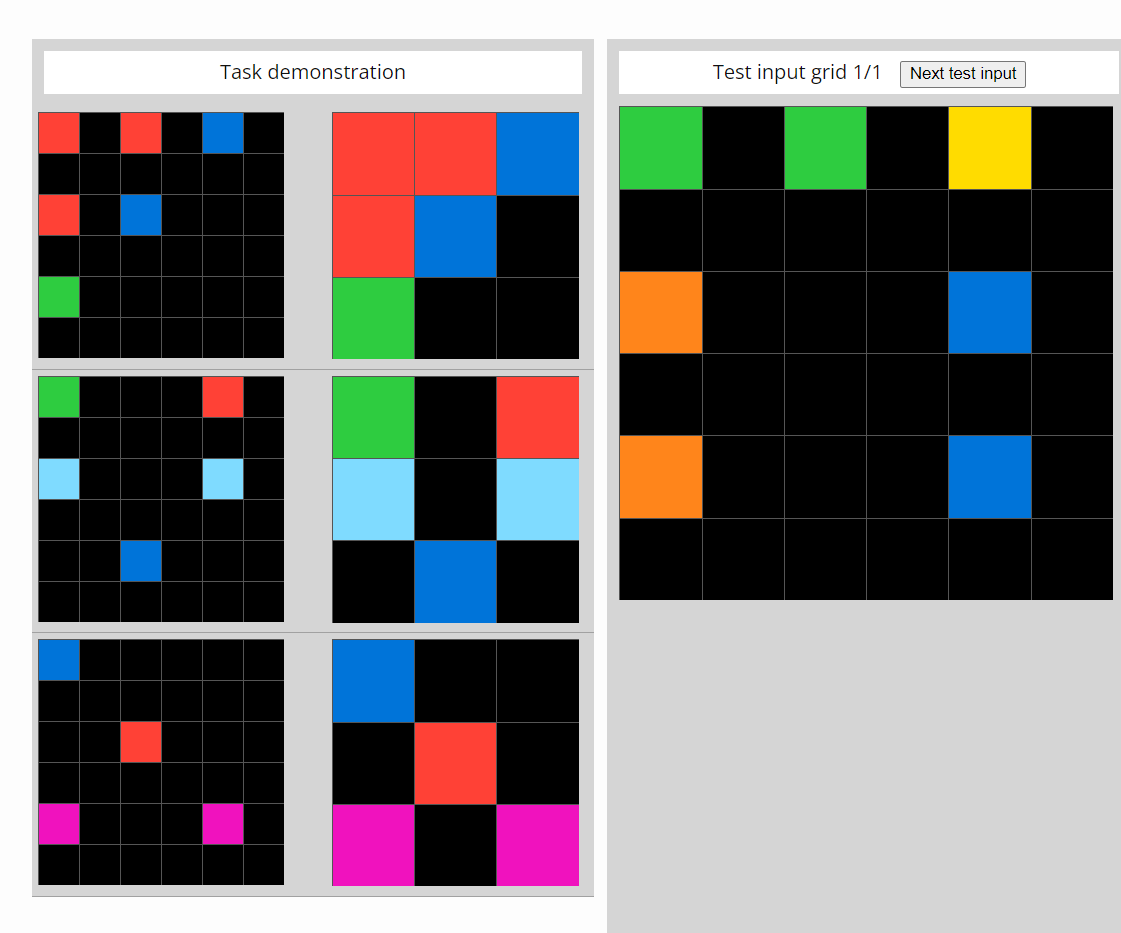
\includegraphics[scale = 0.25]{solved_1.png}
    \vspace{\baselineskip}\vspace{\baselineskip}
    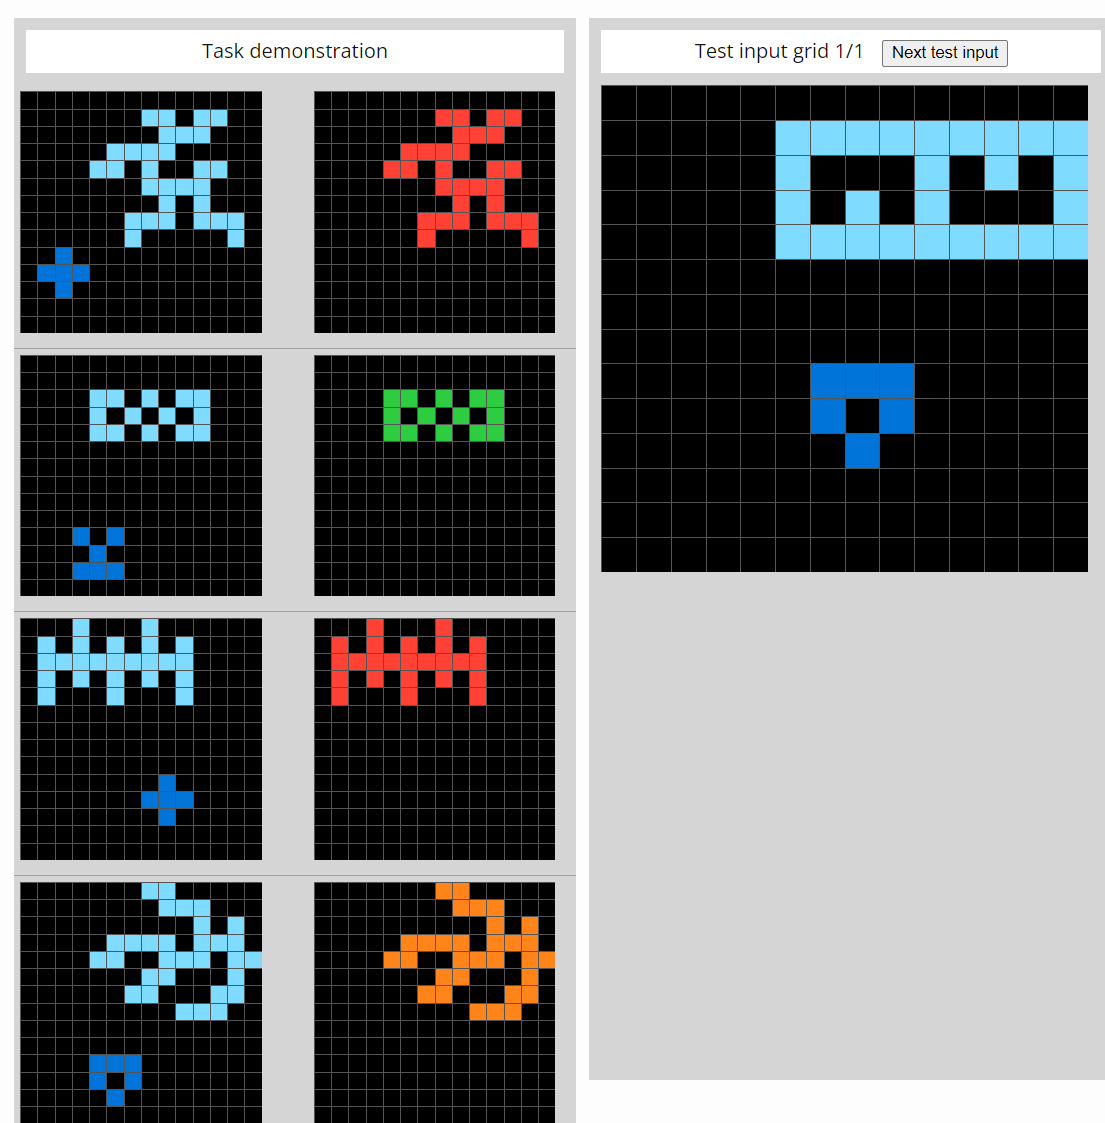
\includegraphics[scale = 0.25]{solved_2.png}
    \vspace{\baselineskip}\vspace{\baselineskip}
    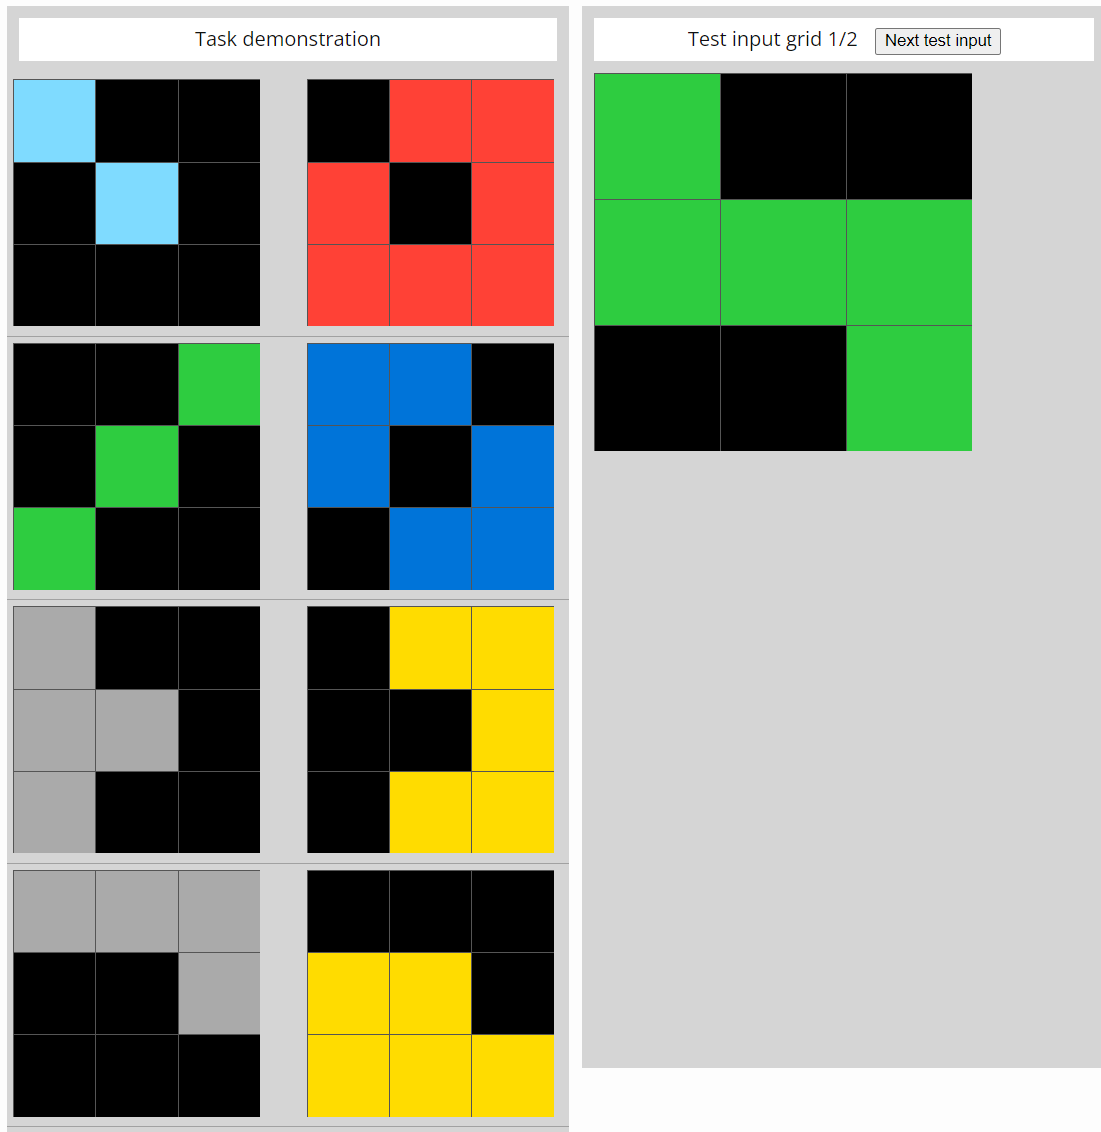
\includegraphics[scale = 0.25]{solved_3.png}
    \vspace{\baselineskip}\vspace{\baselineskip}
    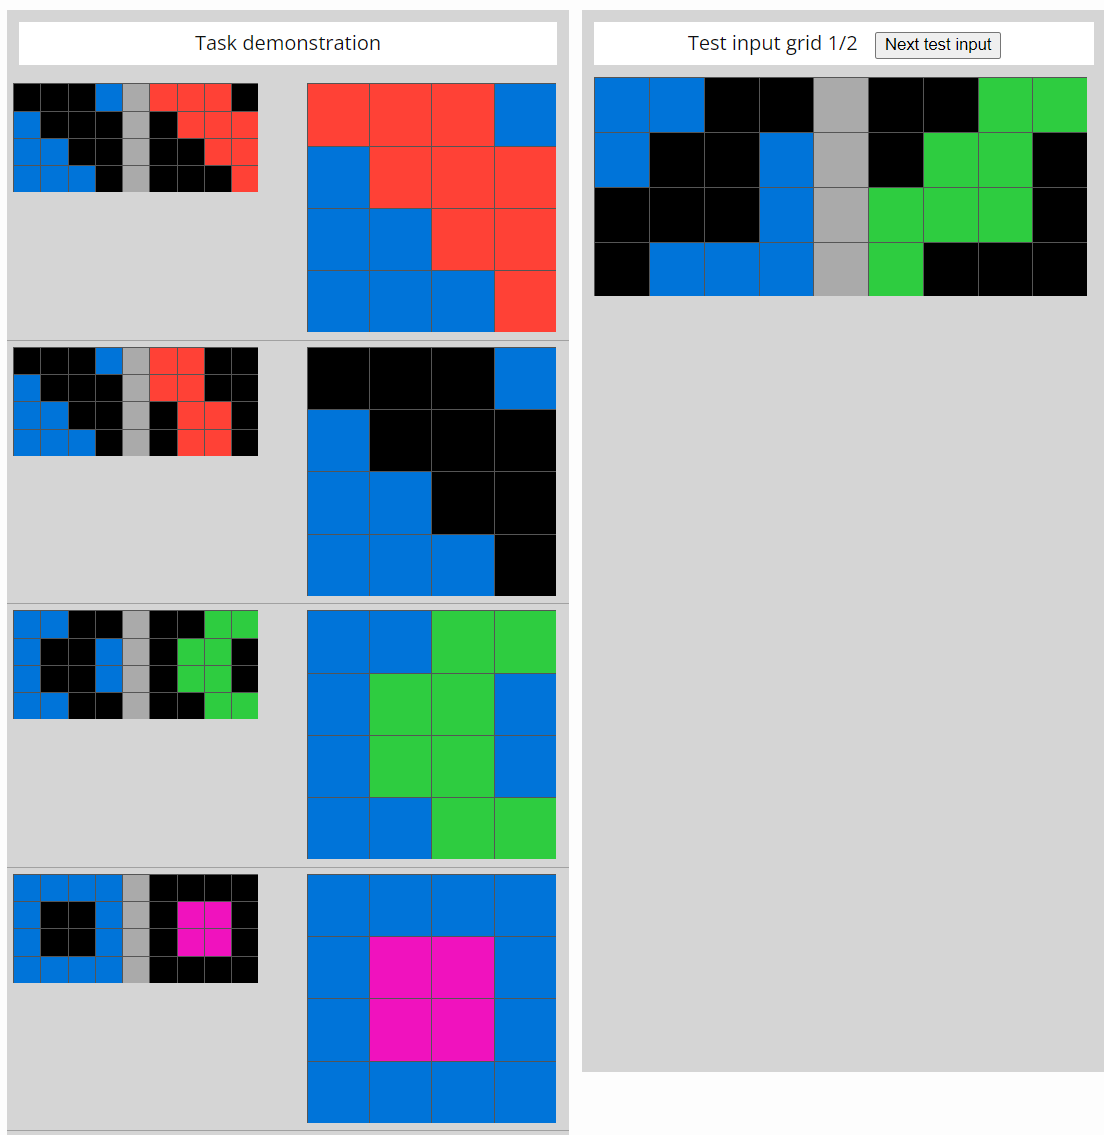
\includegraphics[scale = 0.25]{solved_4.png}
\end{center}

\bigskip

I will go over why my algorithm was able to solve these.
\begin{enumerate}
    \item This is a simple compression, which is defined in my DSL
    \item This is a color mapping of dark blue to black, AND a complex color mapping that depends on the shape of the dark blue object in the input. My algorithm cannot infer this, so it must've made a lucky guess.
    \item The transformation here seems to be a compound color mapping, where black maps to different colors based on what color is shown in the input. My algorithm cannot infer this transformation, so it must've gotten lucky and inferred that black maps to blue, which would be correct for this test case.
    \item This is another transformation that my algorithm cannot infer, so it must've gotten lucky and arbitrarily used the 3rd training pair to infer a transformation of [ lhalf, colormap(black, green) ], which works for the given test input. 
\end{enumerate}

\bigskip

So my algorithm only functions properly for 1 out of 400 cases, but it sometimes gets lucky on another 3. Given this, I will propose some improvements that can be made to my algorithm for future iterations:

\begin{enumerate}
    \item Each transformation inferred from a testing pair gets a ``vote'', so if the same transformation is inferred from two different testing pairs, then it is more likely to be selected.

    \item Add more complex color mapping symbols to the DSL. 3 out of 4 of the problems that I got correct here included color mapping, so it seems that color mapping is the most important thing in the DSL.

    \item Drop some symbols from the DSL that aren't often used so that I can search deeper with a smaller DSL of more useful symbols.

    \item Add support for object segmenting and object-specific transformations.

    \item Infer a transformation from all the input pairs holistically instead of each one individually. This would be helpful for scenarios when black maps to blue only if green appears in the input, for example.

    \item Break ties between competing transformations using similarity weights. This would cause my algorithm to infer transformations that are more simple and thus more plausible.
\end{enumerate}

% \section{Results}
% Lorem Ipsum Results

% \section{Discussion}
% Lorem Ipsum Discussion

% \section{Conclusion}
% Lorem Ipsum Conclusion

% \section{Future Works}
% Lorem Ipsum Future Works

\bibliography{sources}

\end{document}
